\documentclass{article}

\usepackage{hyperref}

% Below will configure hyperlink colors
\hypersetup{
    colorlinks=true,
    linkcolor=blue,
    filecolor=blue,
    urlcolor=blue,
}
\urlstyle{same}

\usepackage{enumitem}

% Below package is for precise positioning of images
\usepackage{float}
\usepackage{color}

% Below package is for syntax highlighted code
\usepackage{minted}
% Below set global setting fro minted package like line wraps and frame
\setminted{breaklines, frame=single}

% Below package is for including images
\usepackage{graphicx}
\usepackage[a4paper, inner=1.5cm, outer=3cm, top=2cm,bottom=3cm, bindingoffset=1cm]{geometry}
\setlength{\parskip}{.5em}

% The LaTeX graphics/graphicx package uses the first dot to find the extension. Package grffile changes this algorithm. This helps in including images files whose name contains more than 1 dot
\usepackage{grffile}


% Below package will create headings
%\pagestyle{headings}

% Below package will used to specify captions like "Figure 1: Nice Figure" in minipages using \captionof{figure}{Nice Figure}
\usepackage{caption}
\usepackage{hypcap} %This is needed for some warning in minipages


\begin{document}
\begin{titlepage}
   \vspace*{\stretch{1.0}}
   \begin{center}
      \Large\textsc{How to get started in hacking OpenJDK?}\\
      \vspace{5mm}
      \Large\textit{Vineel Kumar Reddy Kovvuri}\\
      \url{http://vineelkumarreddy.com}\\
   \end{center}
   \vspace*{\stretch{2.0}}
\end{titlepage}

\tableofcontents

\newpage
\section{Introduction}
This blog post is not about internals of JDK(Java Development Kit), But a mere documentation for people who want to get started. JDK is open sourced a long time ago. The reference implementation of Java is now based on \href{http://openjdk.java.net/}{OpenJDK}. So any one interested in it can get the source code and play with it. Here on, when I refer to JDK it means all the components including Java class libraries/JVM(Hotspot)/Java Compiler. In this post, I will walk you in getting and building the latest JDK 9 sources.

\section{How do I get the source code?}
All the components of JDK 9 are from http://hg.openjdk.java.net/jdk9/ . OpenJDK is under Mercurial. For any one familiar with Git, this is no different. Below is the layout of repositories in JDK 9 OpenJDK forest.


\begin{enumerate}[noitemsep]
\item dev - top-level umbrella project for all the sub projects
    \begin{enumerate}[noitemsep]
    \item corba - Not my interest
    \item hotspot - The Java Virtual Machine implementation. JIT/GC go here
    \item jaxp - Not my interest
    \item jaxws - Not my interest
    \item jdk - The Java class libraries including native JNI implementation go here
    \item langtools - The Java compiler and other tools go here
    \item nashorn - Not my interest
    \end{enumerate}
\end{enumerate}

There are multiple ways to get the code. The easiest being, first clone the umbrella 'dev' project and run get\_source.sh to pull all other repositories.

hg clone http://hg.openjdk.java.net/jdk9/dev 9dev

cd 9dev

sh ./get\_source.sh

Once done you should see below directory structure.

\begin{figure}[H]
\centering
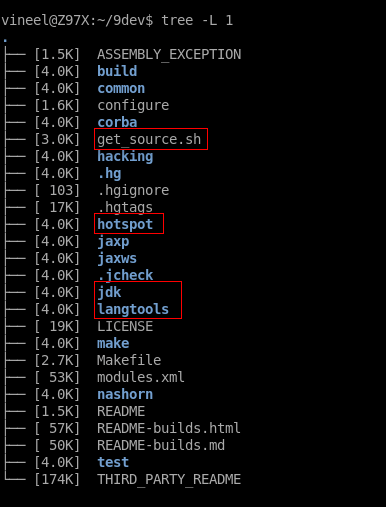
\includegraphics[width=\textwidth]{OpenJDK-1.png}
\caption{}
\end{figure}

\section{How do I build it?}
Building OpenJDK is straight forward too, The only precursor is to get the dependencies. The OpenJDK’s Adopt OpenJDK project has already documented the dependencies here, It’s a matter of sudo apt-get install ….
Run below commands to build the source code. \newline
\newline
bash ./configure \#Setup the environment \newline
make all \#build the entire forest

\begin{figure}[H]
\centering
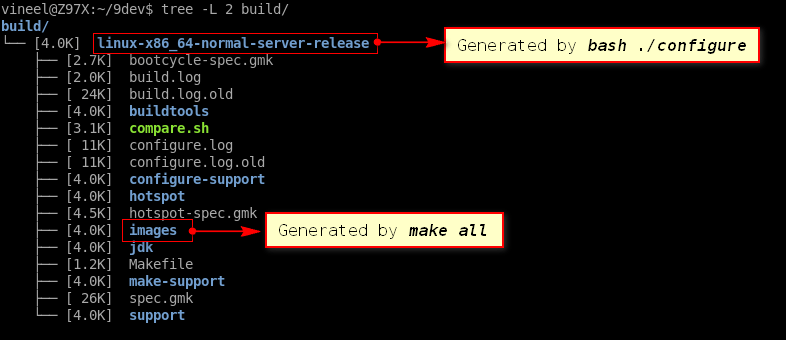
\includegraphics[width=\textwidth]{OpenJDK-2.png}
\caption{OpenJDK build directory after running bash ./configure}
\end{figure}

\begin{figure}[H]
\centering
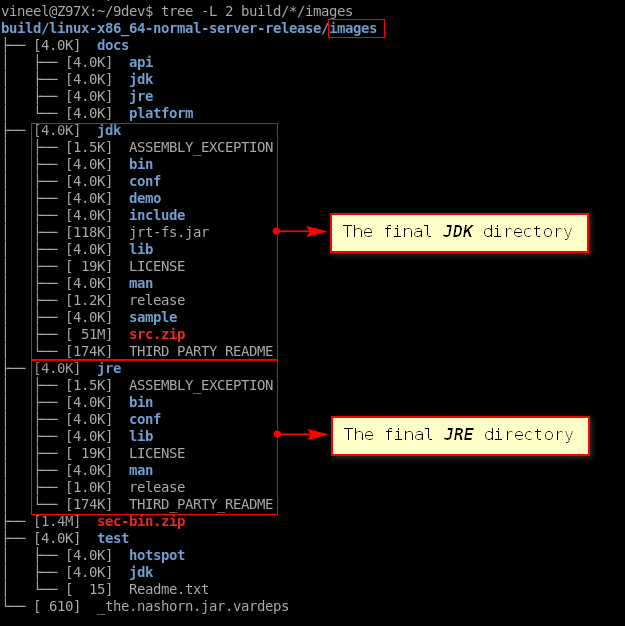
\includegraphics[width=\textwidth]{OpenJDK-3.png}
\caption{OpenJDK images directory after running make all}
\end{figure}

\section{How do I hack it?}
Now its all yours! This is where the fun begins, Even though OpenJDK sources are highly organized, you might need the help of some tools to get around with it. My favorite tool of choice for any source code exploration is OpenGrok, I have my local OpenGrok instance setup.
\begin{figure}[H]
\centering
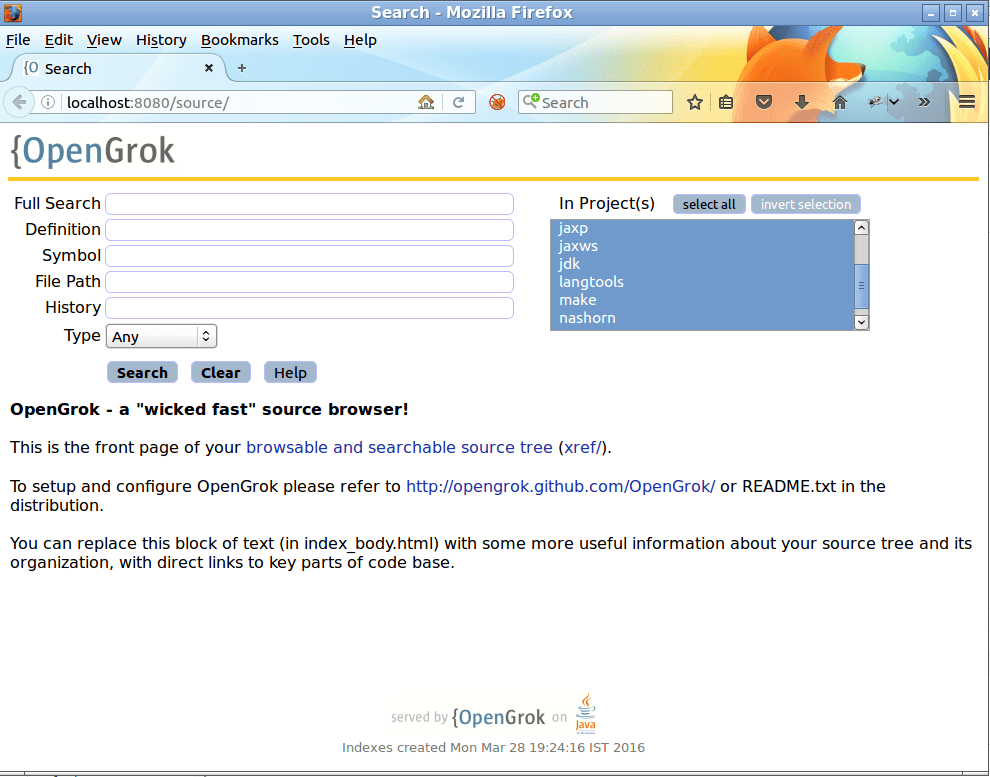
\includegraphics[width=\textwidth]{OpenJDK-4.png}
\caption{}
\end{figure}
Since images/jdk/bin/java is the binary which executes your class files. I wanted to locate the code for it, so that, I can see where the rabbit hole is leading to(essentially in to hotspot) :), The right way to find out is to decipher the build system to understand how things are getting build and from where they are getting build. I really really! don’t want to explore the build system now. So, Its time to wear my black hat and roll up some reverse engineering skills!

With the help of objdump I disassembled the jdk/bin/java binary and looked for symbols, specifically in its main function. Once I know some candidate symbols, I can get to the code from OpenGrok. So below is the disassembled view of main function of the java binary. This function is in turn making calls to JLI\_* apis. So I selected JLI\_PreprocessArg as my candidate symbol.
\begin{figure}[H]
\centering
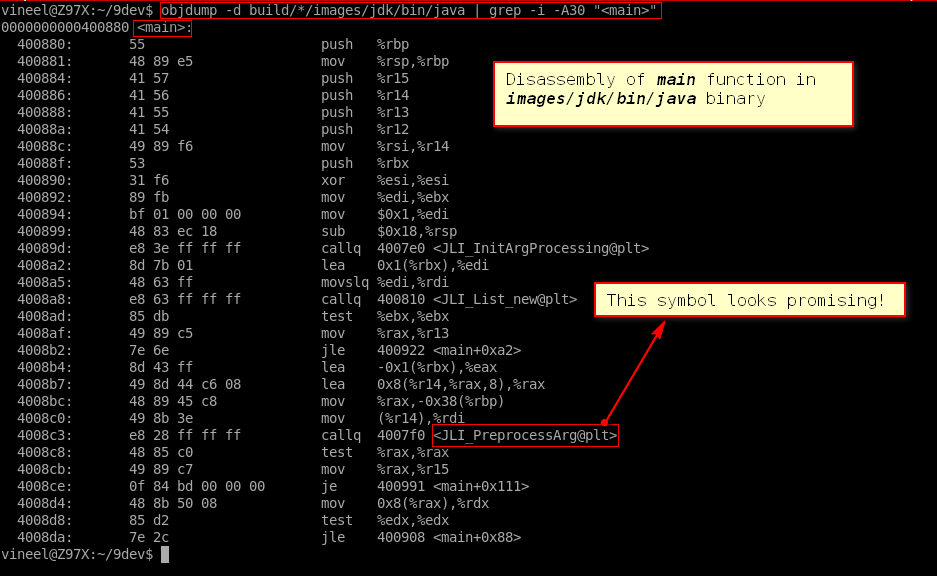
\includegraphics[width=\textwidth]{OpenJDK-5.png}
\caption{}
\end{figure}
Now searching for the symbol JLI\_PreprocessArg in OpenGrok found the source code for jdk/bin/java!
\begin{figure}[H]
\centering
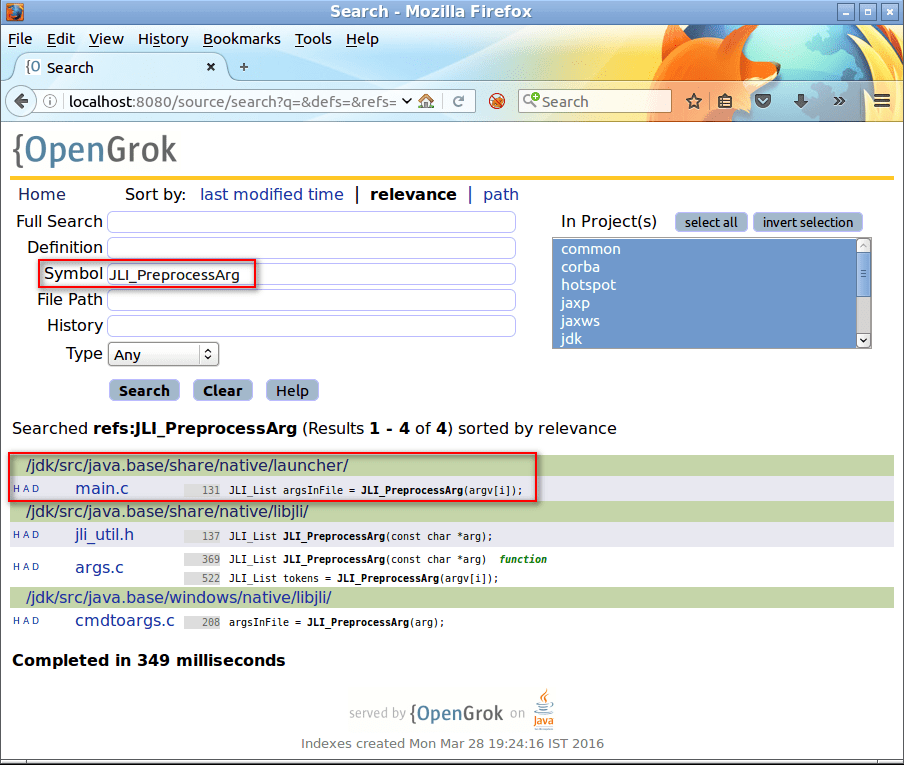
\includegraphics[width=\textwidth]{OpenJDK-6.png}
\caption{}
\end{figure}
\begin{figure}[H]
\centering
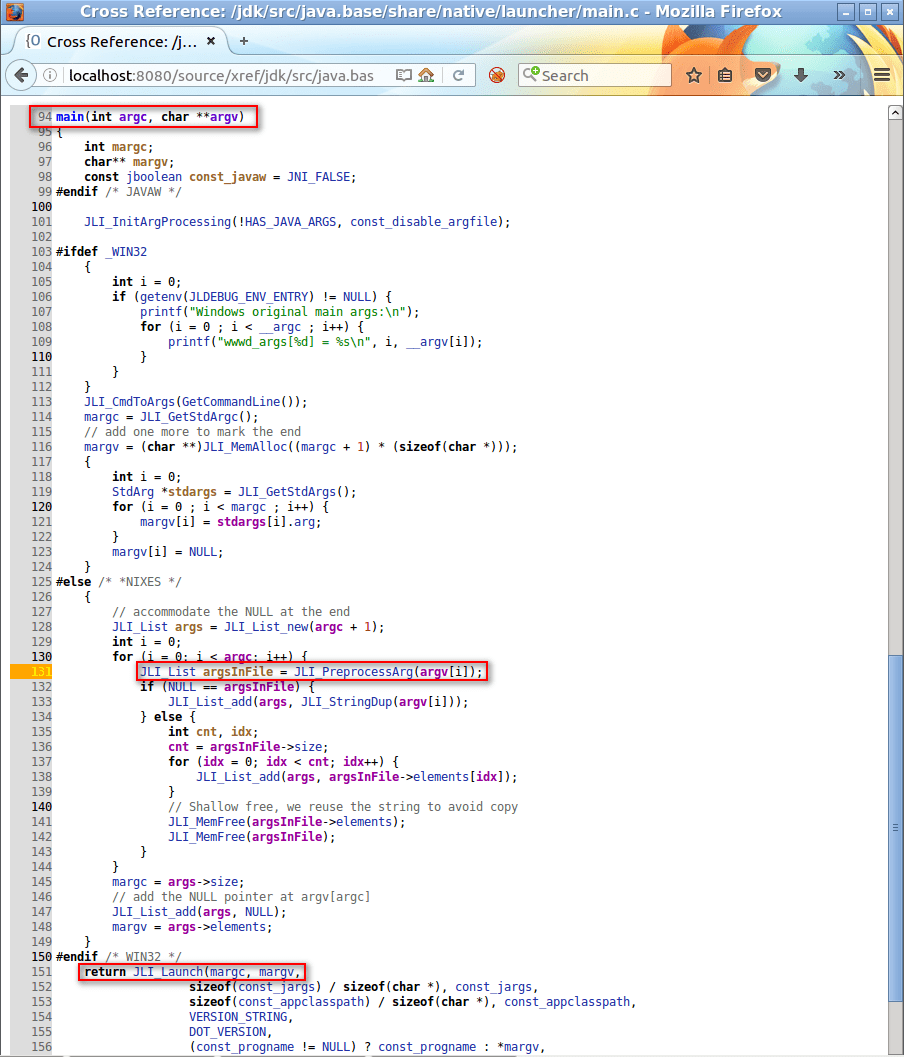
\includegraphics[width=\textwidth]{OpenJDK-7.png}
\caption{Inside main.c}
\end{figure}
To double confirm, I have added a print message and did the make all and it indeed worked as expected! You could see my print when I execute java from the command line in the right side window.
\begin{figure}[H]
\centering
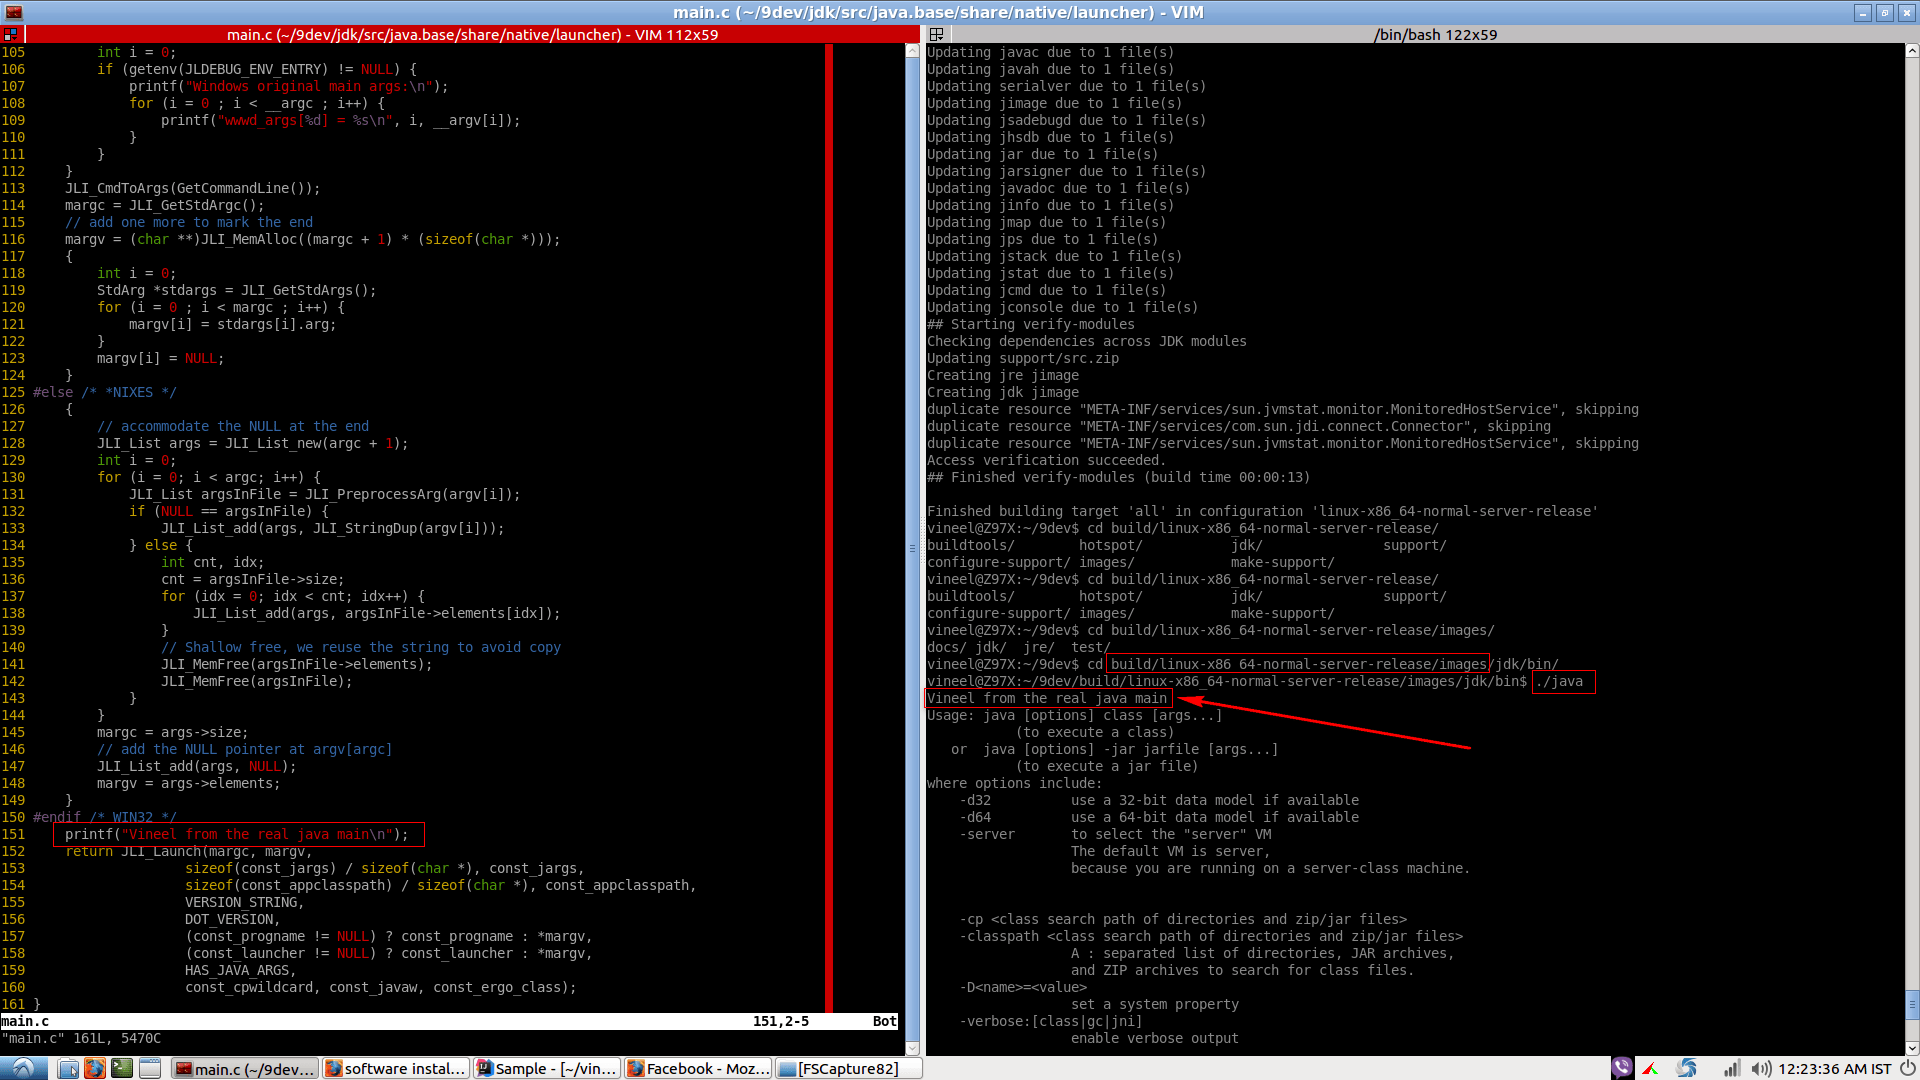
\includegraphics[width=\textwidth]{OpenJDK-8.png}
\caption{Inside main.c}
\end{figure}
\section{References}
\begin{enumerate}[noitemsep]
\item The OpenJDK Developers' Guide - \url{http://openjdk.java.net/guide/}
\end{enumerate}
\end{document}
